% !TEX program = xelatex
\documentclass[11pt]{article}
\usepackage[margin=1in]{geometry}
\usepackage{nopageno} % no page numbers
\usepackage{setspace}

\usepackage{graphicx}
\graphicspath{ {./graphics/} }
\usepackage[dvipsnames]{xcolor}
\definecolor{CrispBlue}{HTML}{0176AE}

\usepackage{fontspec}
\usepackage{tcolorbox}
\usepackage{etoolbox}
\BeforeBeginEnvironment{verbatim*}{\begin{tcolorbox}[colback=CrispBlue!5!white,colframe=CrispBlue!75!black]}%
\AfterEndEnvironment{verbatim*}{\end{tcolorbox}}%

\usepackage{hyperref}
\hypersetup{
    colorlinks,
    citecolor=black,
    filecolor=black,
    linkcolor=black,
    urlcolor=black
}

\usepackage{subcaption}
\setlength{\parindent}{0pt}
\setlength{\parskip}{1em}

\usepackage{tocloft}
\renewcommand{\cftpartleader}{\cftdotfill{\cftdotsep}}
\renewcommand{\cftsecleader}{\cftdotfill{\cftdotsep}}

\usepackage[shortlabels]{enumitem}

\usepackage{fancyhdr}
\pagestyle{fancy}
\fancyhf{}
\lhead{ECE 517: Machine Learning}
\rhead{Assignment 7.1}
\rfoot{Page \thepage}

\usepackage{amsmath,amsfonts,amssymb}
\usepackage{bm}
\usepackage{mathtools}

\renewcommand{\listfigurename}{List of Figures}

\begin{document}
\setmainfont{SF Pro Text}
\setsansfont{SF Pro Text}
\setmonofont{SF Mono}
\renewcommand{\familydefault}{\sfdefault}

\thispagestyle{empty}
\begin{titlepage}
\vspace*{\fill}
\begin{center}
\textsc{\Huge{ECE 517: Machine Learning}}\\[3em]
\textsc{\LARGE Assignment 7.1: Gaussian Processes}\\[6em]
\textsc{\Large David Kirby -- 101652098 -- davidkirby@unm.edu}\\[3em]
\textsc{\Large Fall 2021}
\end{center}
\vfill
\begin{figure}[h]
\begin{subfigure}{0.5\textwidth}

\includegraphics[width=0.25\linewidth]{learning.png}
\end{subfigure}
\begin{subfigure}{0.6\textwidth}\hspace{1em}

\includegraphics[width=0.8\linewidth]{new-soe-logo.png}
\end{subfigure}
\end{figure}
\end{titlepage}
\setcounter{figure}{0}

\hypersetup{
    linkcolor=CrispBlue,
    urlcolor=CrispBlue,
    breaklinks=true
}

\textbf{GAUSSIAN PROCESSES}

Using the GP software and the script provided with Video 7.4, reproduce the first example of lesson 7.3.

\begin{tcolorbox}[colback=CrispBlue!5!white,colframe=CrispBlue!75!black,title=Gaussian Process.]\setstretch{1.25}
    This first example is in one dimension and the model that generates the data is:
    
    \begin{equation}
        y_n = 0.5x_n + 0.5 + w_n
    \end{equation}
    
    Where \(x_n\) is a uniform random variable between 0 and 1, \(w\) is Gaussian noise with variance \(\sigma^2\). The standard deviation is 0.5 and for the training, we take 50 samples from this linear model. For the test, we have 10 samples that are uniformly spaced between 0 and 1. In blue, we have the training samples with noise, and in black, we have the regression line with 10 points.

\end{tcolorbox}

\begin{figure}[h!]
    \centering
    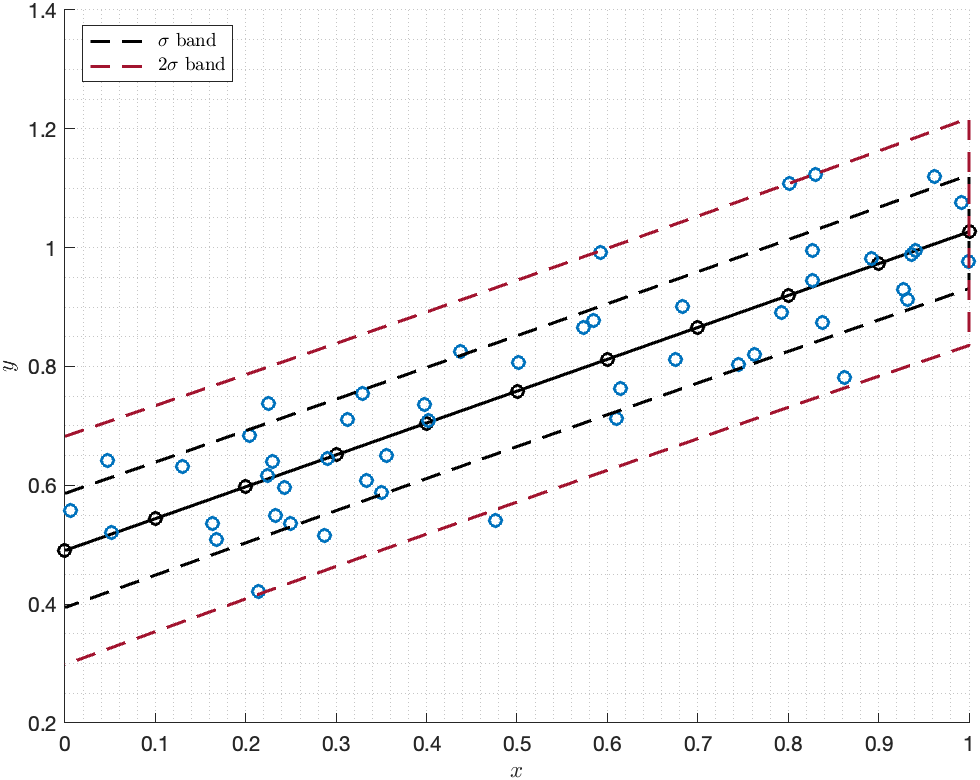
\includegraphics[width=\textwidth]{figure01.png}
    \caption{Linear GP regression over the linear model \( y_n = 0.5x_n + 0.5 + w_n\).}
    \label{fig:fig01}
\end{figure}


\end{document}